\documentclass[handout]{beamer}
\usepackage{pgfpages}
%\documentclass{beamer}
%\usepackage{beamerthemesplit}

\def\ce#1{\centerline{#1}}
\def\no{\noindent} 
\def\nl{\newline}
% -------
 \def\cblack{\color{black}}
 \def\cb{\color{blue}}
 \def\cred{\color{red}}
 \def\cy{\color{yellow}}
 \def\cg{\color{cyan}}
% -------
 \def\bs{\end{slide}\begin{slide}}
 \def\bi{\begin{itemize}} 
 \def\ei{\end{itemize}}
 \def\i{\item} 
 
\def\t{\theta} 
\def\l{\lambda} 
\def\d{\delta} 

\def\Pr{\mbox{Pr}}
\def\E{\mbox{E}}
\def\Var{\mbox{V}}
\def\ind{\stackrel{ind}{\sim}}
\def\iid{\stackrel{iid}{\sim}}


\title{STA 360/601: Bayesian and Modern Statistics}

\subtitle{Lecture 3:\\Count data, Gamma-Poisson model, \& Posterior summaries}

\author{Jeff Miller}

\institute{Department of Statistical Science, Duke University}

\date{Wednesday, September 3, 2014}

\graphicspath{{figures/}}

\begin{document}

\frame{\titlepage}

%\section[Outline]{}
%\frame{\tableofcontents}


\section{Count data}

\frame{\frametitle{Count data}
    Suppose our data is counts $y_i \in \mathcal{Y} = \{0,1,2,\ldots\}$ for $i=1,\ldots,n$.
    \begin{itemize}[<+-| alert@+>]
        \i e.g., \# friends on facebook, \# website hits per minute, \\
        \# points scored in a game, \# neuron spikes in a given interval,
        \# photons hitting a CCD pixel.
        \i Often, a natural choice of likelihood is Poisson:
        $$L(y; \theta) = \prod_{i=1}^n \frac{\exp(-\theta)\theta^{y_i}}{ y_i! },$$
        assuming conditional independence of the counts given $\theta$.
    \ei 
}


\frame{\frametitle{Sim\'eon Denis Poisson (1781 -- 1840)}
\centerline{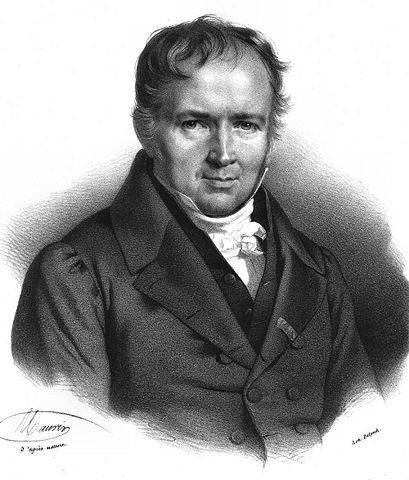
\includegraphics[height=5cm]{Simeon_Poisson.jpg}}
}

\frame{\frametitle{Poisson distribution}
    $Y \sim \mbox{Poisson}(\theta)$ (or $\mbox{Pois}(\t)$), where $\theta>0$, means
         $$\displaystyle\Pr(Y=y\mid \theta) = \frac{\theta^y}{y!}e^{-\theta}.$$
    Notes:
    \begin{itemize}[<+-| alert@+>]
        \i \underline{Mean = Variance:} $\E(Y|\theta)=\Var(Y|\theta)=\theta$.
        \i \underline{Sum of Poissons is Poisson:}\\
            If $Y_i \ind \mbox{Pois}(\theta_i)$ for $i=1,...,n$, then $\sum Y_i \sim \mbox{Pois}(\sum \theta_i)$.
        \i Limit of $\mbox{Binomial}(n,p_n)$ with $p_n=\theta/n$ as $n\to \infty$ is Poisson:
        $${n \choose y} (\theta/n)^y (1-\theta/n)^{n-y} \longrightarrow \frac{\theta^y}{y!}e^{-\theta}$$
        (special case of the ``law of small numbers'').
    \ei 
}

\frame{ \frametitle{Fake real-world example}
    \begin{itemize}[<+-| alert@+>]
        \item You are planning to start a pizza delivery business.
        \item It's essential to know how many orders you will get.
        \item A priori, you think your average number of orders/hour will be around 15--25 (in the evening), but you're not really sure.
        \item To get some data, you stakeout a comparable pizza delivery business over a few evenings, and record how many deliveries they
            make each hour.  Over $n=6$ hours, you observe
            $$y_{1:n} = (16, 10, 22, 14, 19, 18).$$
        \item More data would be nice but you've already spent 6 hours \dots you can use your prior knowledge to help make inferences.
        \item You're happy with a Poisson likelihood, but to do a Bayesian analysis, you also need a prior on $\theta$, the mean \# pizzas/hour.
    \end{itemize}
}

\frame{ \frametitle{Sufficient statistics for Poisson}
    \begin{itemize}[<+-| alert@+>]
        \i The likelihood simplifies:
        $$ L(y; \theta) = \prod_{i=1}^n \frac{ \theta^{y_i} \exp(-\theta) }{ y_i! } = C(y)\, \theta^{\sum_{i=1}^n y_i }\exp(-n\theta). $$
        \i $S(y)=\sum y_i$ is a {\em sufficient statistic}: as a function of $\t$ the likelihood depends only on $S(y)$,
        up to a constant of proportionality $C(y)$.
        %\i If we have a prior on $\t$, this says $\t\perp y | S(y)$.
        \i \underline{Intuitive interpretation:} $S(y)$ contains all the information about $\theta$ present in the data.
        ``$Y\perp \t|S(Y)$''
        \i \underline{Practical upshot:} We don't need to store the individual counts $y_1,\ldots,y_n$ --- just keep the sum (and $n$).
        \i As a function of $\theta$, $L(y; \theta) \propto \theta^{S(y)}\exp(-n\theta)$.  The Gamma distribution gives us a conjugate prior.
    \end{itemize}
}


\section{Gamma-Poisson model}

\frame{ \frametitle{Gamma distribution}
    $\theta \sim \mbox{Ga}(a,b)$ (where $a,b>0$) means the pdf of $\theta$ is 
        $$\mbox{Ga}(\theta;a,b)=\frac{ b^a }{ \Gamma(a) } \theta^{a-1} \exp(-b\theta).$$ 
    Notes:
    \begin{itemize}[<+-| alert@+>]
        \i $a$ = ``shape'', $b$ = ``rate''.
        \i \underline{Achtung!} Alternate parametrizations are in common use.
        \i $\E(\theta) = a/b$, \quad $\Var(\theta)=a/b^2$
        \i To obtain a given prior mean and std.\ dev.\ $\mu>0$ and $\sigma>0$,
            we can solve for $a,b$ s.t.\ $\mu = a/b$ and $\sigma^2 = a/b^2$.
        \i \underline{Sum of Gammas:}\\
            If $\theta_i \ind \mbox{Ga}(a_i,b)$ for $i=1,\ldots,n$, then $\sum \theta_i \sim \mbox{Ga}(\sum a_i,b)$.
        \i \underline{Scaling:}\\
            If $\theta \sim \mbox{Ga}(a,b)$ and $c>0$, then $c\theta \sim \mbox{Ga}(a,b/c)$.
    \end{itemize}
}

% Mention relationships with exponential \& chisquare as well as some basic gamma properties & dirichlet perhaps

\frame{ \frametitle{Some Gamma densities for various $a,b$}
%\centerline{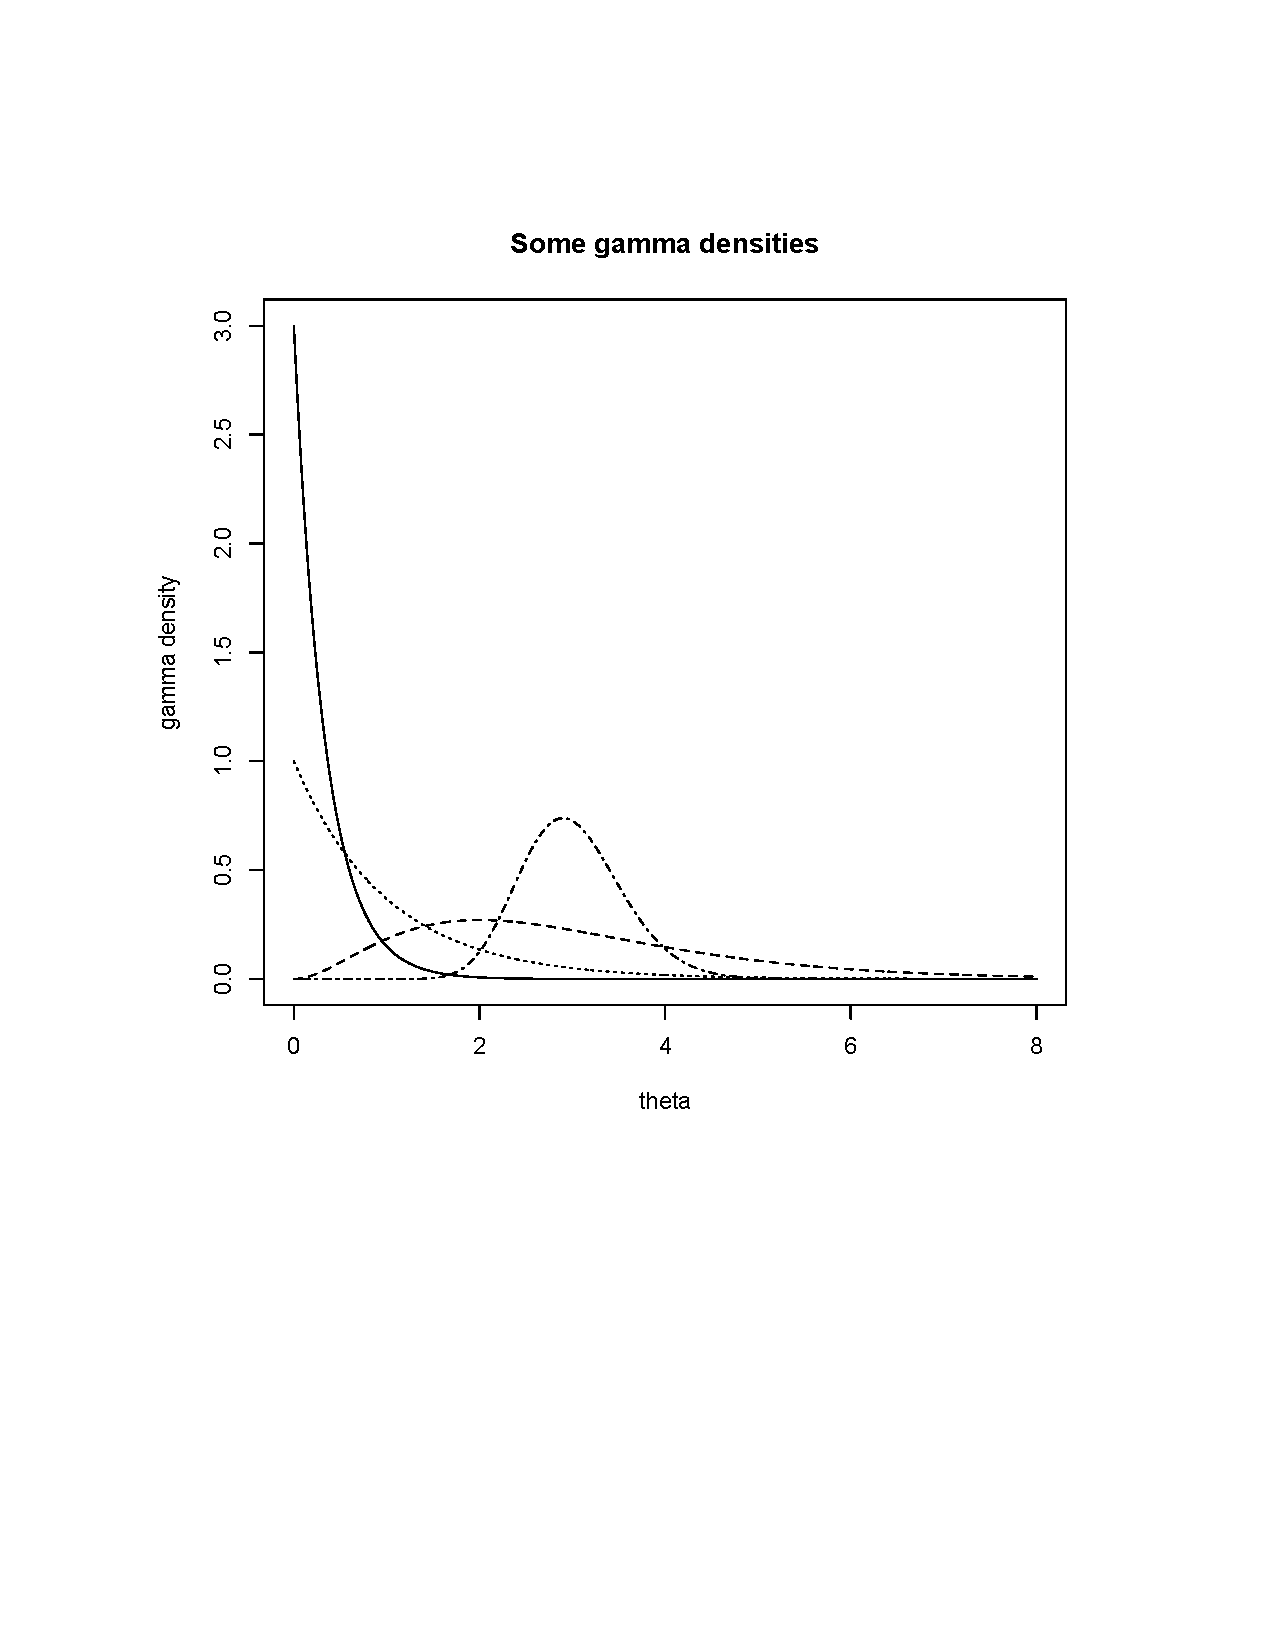
\includegraphics[trim=0 4cm 0 2cm, clip=true, height=10cm]{gamma_densities.pdf}}
    \centerline{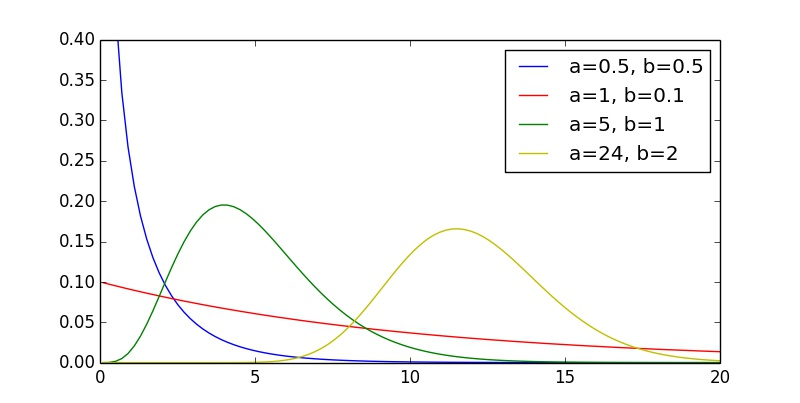
\includegraphics[height=5cm]{gammas.jpg}}
}


\frame{ \frametitle{Pizza prior}
    Back to pizza \dots
    \begin{itemize}[<+-| alert@+>]
        \item You need to put a prior on $\theta$ (mean \# pizzas sold per hour).
        \item For convenience, you choose a Gamma prior.
        \item Based on your (somewhat uncertain) prior belief, you choose $\mu=20$ and $\sigma=8$, thus $b=\mu/\sigma^2=0.3125\approx 0.31$ and $a=b\mu=6.25$.
    \end{itemize}

    ~\\
    \centerline{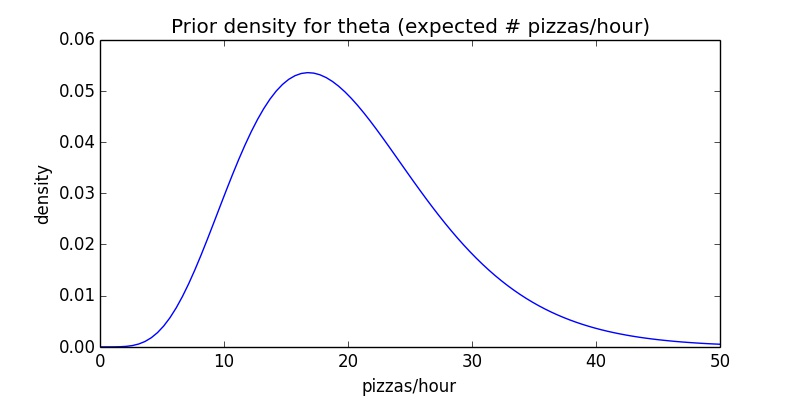
\includegraphics[height=4cm]{prior.jpg}}
}


\frame{ \frametitle{Posterior of Gamma-Poisson model}
\begin{align*}
\pi( \theta | y ) 
& \propto \mbox{likelihood} \times \mbox{prior} = L(y;\theta) \mbox{Ga}(\theta;a,b) \\
& \propto \theta^{S(y)} \exp( -n\theta)\, \theta^{a-1} \exp(-b\theta) \\
& \propto \theta^{a + S(y) - 1} \exp\big(-\theta(b+n)\big) \\
& \propto \mbox{Ga}(\theta; \widehat{a}, \widehat{b} ),
\end{align*}
where $\widehat{a}=a + S(y)$, $\widehat{b} = b + n$, and $S(y)=\sum_i y_i$.

\begin{itemize}[<+-| alert@+>]
\item Can roughly interpret $b$ as prior ``sample size''.
\item \underline{Posterior mean:} (convex combo of prior \& sample means) \\
    $$\E( \theta | y) = \frac{a+\sum y_i}{b + n} = \frac{b}{b+n} a/b + \frac{n}{b+n}\overline{y}.$$
\item $\E(\theta|y) \approx \overline{y}=\frac{1}{n}\sum y_i$ for large $n$.
\item \underline{Posterior variance:} $\Var( \theta | y) = (a+\sum y_i)/(b+n)^2 \approx \overline{y}/n$ for large $n$.
\end{itemize}
}


\frame{ \frametitle{Pizza posterior}
    \begin{itemize}[<+-| alert@+>]
        \item Your angel investor just called, and he wants to know how many pizzas you expect to sell per hour, on average?
        \item And how certain are you about that?
        %\item Likelihood: $\mbox{Pois}(\theta)$, Prior: $\mbox{Ga}(\theta; a,b)$ with $a=6.25$, $b=0.3125$.
        %\item Data: $y_{1:n} = (16, 10, 22, 14, 19, 18)$, $S(y) = \sum y_i = 99$.
    \item Posterior: $\mbox{Ga}(\theta; \widehat{a}, \widehat{b} )$ with $\widehat{a}=a + S(y)=105.25$, $\widehat{b} = b + n \approx 6.31$.
        \centerline{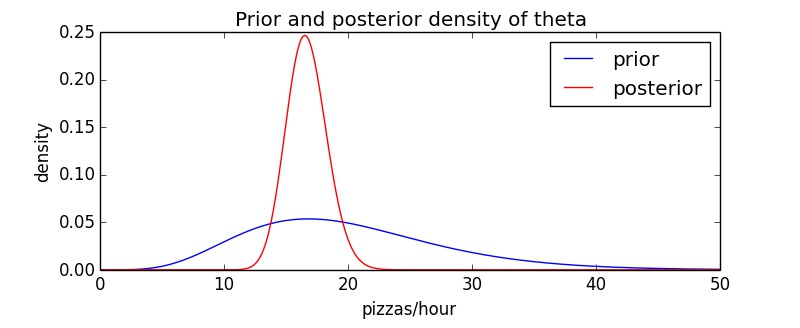
\includegraphics[height=4cm]{posterior.jpg}}
        \item Your investor never took Bayesian statistics, so you need to summarize this posterior.
    \end{itemize}
}


\section{Posterior Intervals}

\frame{ \frametitle{Posterior Intervals}
 %Summary ``estimates'' of $\t$ 
\begin{itemize}
    \item \underline{Names:} Credible intervals/sets, Bayesian confidence intervals/sets, Posterior intervals.
    \item \underline{Central intervals (equal tails):}\\
        $[\ell(y),u(y)]$ is a $100(1-\alpha)\%$ central credible interval if
        $$\Pr(\theta<\ell(y)|y)=\alpha/2, \quad \Pr(\theta>u(y)|y)=\alpha/2.$$
        E.g., for a 95\% interval, choose $\alpha=0.05$.
    \item \underline{Highest posterior density (HPD) set:}\\
        A set $A(y)$ is a $100(1-\alpha)\%$ HPD set if
        $$\Pr(\theta\in A(y)|y)=1-\alpha$$
        and $\pi(\t_1|y)\geq \pi(\t_2|y)$ for any $\t_1\in A(y)$, $\t_2\not\in A(y)$.
\end{itemize}
}

\frame{ \frametitle{Pizza interval}
 %Summary ``estimates'' of $\t$ 
In our example, $[13.6, 20.0]$ is the 95\% central credible interval:
\centerline{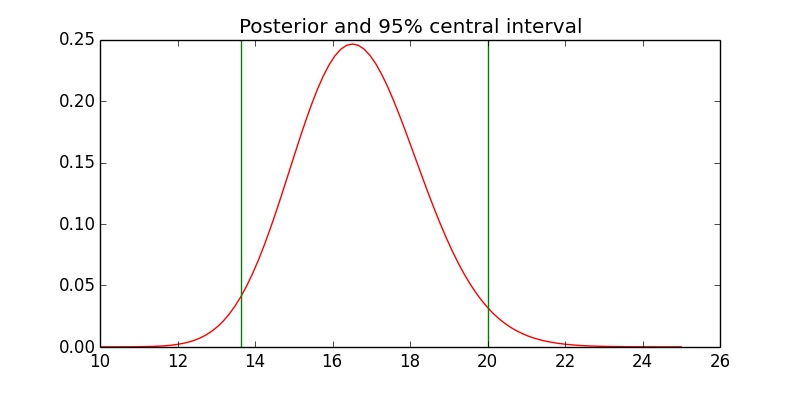
\includegraphics[height=4cm]{interval.jpg}}
\begin{itemize}
    \item You can tell your investor that \underline{your belief} is that there is a 95\% probability
        that a business like yours sells between 13.6 and 20 pizzas/hour, on average.
    \item (Note: This is a statement about the mean, not the \# in any given hour.)
\end{itemize}
}

\frame{ \frametitle{Bayesian vs.\ Frequentist intervals}
\begin{itemize}
    \item Bayesian confidence intervals (credible intervals) are different than frequentist confidence intervals.
    \item \underline{Bayesian:}\\
        $\Pr(\ell(y)<\theta<u(y)\mid y)=0.95$ for any $y$. ($\theta$ is random)
    \item \underline{Frequentist:}\\
        $\Pr(\ell(Y)<\theta<u(Y)\mid \theta)=0.95$ for any $\theta$. ($Y$ is random)
    \item If you had constructed a frequentist interval, you would tell your investor that 95\% of the time,
        an analysis like yours would yield an interval containing the true value.
    \item Credible intervals do not always guarantee coverage in the frequentist sense --- however, they do asymptotically (see Hoff,
        p.\ 41).  Many frequentist methods also only guarantee coverage
        asymptotically. % (e.g., Chi-square or Normal approx.).
\end{itemize}
}


\frame{ \frametitle{Hiring --- a decision problem}
    \begin{itemize}[<+-| alert@+>]
        \item Your investor is satisfied for now, but you have a new problem:\\
              How many delivery people should you have working each evening?
        \item Each deliverer costs you $c=14$ dollars/hour.
        \item Each deliverer can handle a maximum of $m=6$ orders/hour.
        \item If you have $d$ deliverers, you can handle $m d$ orders/hour.
        \item Your business guarantees delivery within 30 minutes, so for each order in excess of $m d$ you lose \$20.
        \item Loss function (dollars/hour):
            $\mathcal{L}(d,y) = c d + 20\max(y-m d,0) = 14 d + 20\max(y - 6 d,0)$.
        \item Bayes risk: $R(d) = \E(\mathcal{L}(d,y_{n+1}) | y_{1:n})$.
        \item To compute this, you need the posterior predictive $y_{n+1}|y_{1:n}$.
    \end{itemize}
}


\frame{ \frametitle{Prediction}
We need the posterior predictive pmf $f(y_{n+1}|y_{1:n})$.  To simplify notation, write $y$ for $y_{n+1}$.
\begin{align*}
f(y|y_{1:n}) & = \int \mbox{Pois}(y; \theta) \mbox{Ga}( \theta; \widehat{a}, \widehat{b})d\theta \\
& = \frac{ \widehat{b}^{\widehat{a}} }{ y! \Gamma(\widehat{a}) } \int_0^\infty
    \theta^{\widehat{a}+y-1} \exp\big( -\theta(\widehat{b}+1) \big)d\theta \\
& = \frac{ \widehat{b}^{\widehat{a}} }{ y! \Gamma(\widehat{a}) } \frac{\Gamma(\widehat{a}+y)}{(\widehat{b}+1)^{\widehat{a}+y}}  \\
& = \frac{ \Gamma( \widehat{a}+y ) }{ \Gamma(y+1)\Gamma(\widehat{a}) }\bigg( \frac{\widehat{b}}{ \widehat{b}+1 } \bigg)^{\widehat{a}}
\bigg( \frac{1}{\widehat{b}+1} \bigg)^y.
\end{align*}
This is the negative-binomial dist, $\mbox{NegBinom}(\widehat{a},1/(\widehat{b}+1))$.
}

\frame{ \frametitle{Prediction (continued) }
\begin{itemize}[<+-| alert@+>]
\item In marginalizing $\theta$ out of the Poisson($y; \theta$) likelihood over a gamma distribution, we obtain a negative-binomial.
%\item It is an \emph{over-dispersed} generalization of the Poisson.
\item The negative-binomial distribution also models count data, but has somewhat more flexibility, with two parameters, allowing control of mean and variance.
\item For $(y | y_{1:n}) \sim \mbox{NegBinom}(\widehat{a},1/(\widehat{b}+1))$, we have 
\begin{align*}
\E(y | y_{1:n}) & = \widehat{a}/\widehat{b} = \E( \theta |y_{1:n}) = \mbox{Posterior mean} \\
\Var(y | y_{1:n}) & = \frac{ \widehat{a}(\widehat{b}+1) }{ \widehat{b}^2 } = \E( \theta | y_{1:n})\bigg(\frac{\widehat{b}+1}{\widehat{b}} \bigg).
\end{align*}
So, the variance is larger than the mean by an amount determined by $\widehat{b}$.

\end{itemize}
}

\frame{ \frametitle{Pizza prediction}
    The posterior predictive distribution of the number of pizza orders in a given hour is
    $\mbox{NegBinom}(y;\widehat{a},1/(\widehat{b}+1))$.

    ~\\
    \centerline{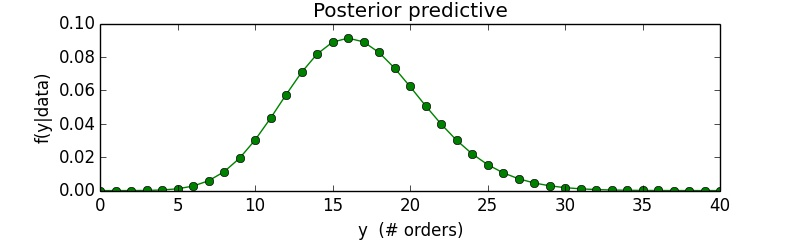
\includegraphics[height=2.6cm]{predictive.jpg}}
    ~\\
    \centerline{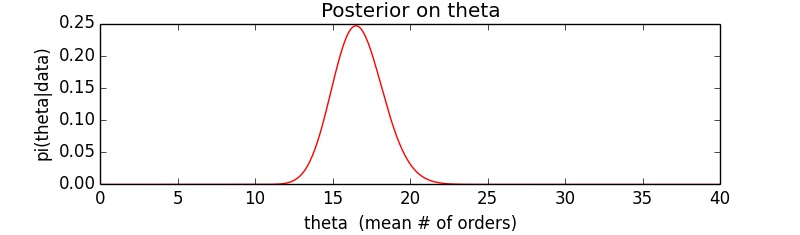
\includegraphics[height=2.5cm]{posterior-alone.jpg}}
}

\frame{ \frametitle{Predictive uncertainty}
\begin{itemize}[<+-| alert@+>]
\item Note that as the sample size $n$ increases, the posterior density for $\theta$ becomes more and more concentrated: \\
  $\Var( \theta | y_{1:n} ) = \widehat{a}/\widehat{b}^2 = (a + \sum_i y_i)/( b + n)^2 \approx \overline{y}/n \to 0$.

\item As we have less uncertainty about $\theta$, the inflation factor $(\widehat{b}+1)/\widehat{b} \to 1$ and the 
predictive density $f(y|y_{1:n}) \to \mbox{Pois}(\overline{y})$.

\item In smaller samples, though, using this approximation can lead one to underestimate predictive variance,
    since it's important to account for uncertainty in $\theta|y_{1:n}$ (not just in $y|\t$).
\end{itemize}
}

\frame{ \frametitle{More on the Negative Binomial}
\begin{itemize}[<+-| alert@+>]
\item Can be derived as the \# successes in a sequence of Bernoulli($p$) trials before $r$ failures occur.

\item This is denoted $Y \sim \mbox{NegBinom}(r, p)$ and the pmf is 
$$\Pr(Y=k) = { k+r-1 \choose  k }(1-p)^r p^k.$$

\item Starting with this, the distribution can be extended to allow noninteger $r \in (0,\infty)$ as 
$$\Pr(Y=k) = \frac{ \Gamma(k+r) }{ \Gamma(k+1)\Gamma(r) }(1-p)^r p^k,$$
which is the form we obtained above as the predictive with $r=\widehat{a}$, $p=1/(\widehat{b}+1)$.

\end{itemize}
}

\frame{ \frametitle{How many deliverers to have?}
    \begin{itemize}[<+-| alert@+>]
        \item Loss function: $\mathcal{L}(d,y) = 14 d + 20\max(y - 6 d,0)$.
        \item Bayes risk: $R(d) = \E(\mathcal{L}(d,y) | y_{1:n})=\sum_y \mathcal{L}(d,y)f(y|y_{1:n})$.
        \item Looks nasty to compute analytically, but it's easy numerically.
        \centerline{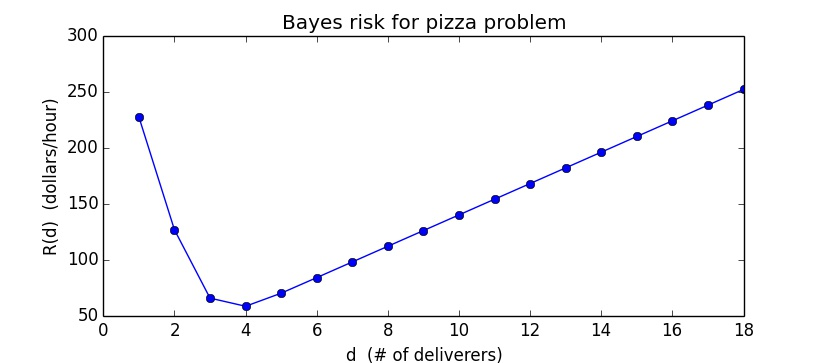
\includegraphics[height=4cm]{risk.jpg}}
        \item If too few, we often have to pay for $>30$ minute deliveries.
        \item If too many, have to pay too much in wages, etc.
    \end{itemize}
}



%% ------------------------------------------------------------

\frame{ \frametitle{Homework exercise}
\begin{itemize}[<+-| alert@+>]
    \item Suppose for subjects $1,\ldots,n$, we observe that $y_i$ is the length of time it takes to perform a task.

    \item Assume $y_i \iid \mbox{Exp}( \theta )$ given $\theta$:
        $$L(y ; \theta) = \prod_{i=1}^n \theta \exp( - \theta y_i )$$
    \item Assume $\theta \sim \mbox{Ga}(a,b)$ a priori.

    \item Calculate the posterior distribution of $\theta$.

    \item Calculate the posterior predictive distribution $f(y_{n+1}|y_{1:n})$.

    \item Describe how this could be used for prediction, including quantification of uncertainty.
\end{itemize}
}





%\frame{\frametitle{References}
    %\begin{itemize}[<+-| alert@+>]
        %\item Peter D.\ Hoff, \emph{A First Course in Bayesian Statistical Methods}, Springer, 2009.
        %\item Rick Durrett, \emph{Probability: Theory and Examples}, Cambridge University Press, 2010.
    %\ei 
%}





 
\end{document}








